
\chapter{QUIC Protocol}\label{chap:02-quic}

This chapter is intended as a summary of the QUIC protocol specification providing sufficent detail
for the design of our implementation. The text is based on the version 29 of the draft specification
documents from June 2020, more specifically on the documents describing the core transport
protocol~\cite{draft-ietf-quic-transport}, TLS integration~\cite{draft-ietf-quic-tls}, and
congestion control mechanism~\cite{draft-ietf-quic-recovery}. Readers familiar with these documents
may skip this chapter.

We will start this chapter by first providing a high-level overview of QUIC, and then provide a more
detailed description of individual parts of the protocol.

\section{Overview of QUIC}

QUIC protocol provides a reliable and secure transport of multiple streams of data over a single
connection\footnote{The ability to transport multiple streams over a single connection is called
  \textit{stream multiplexing}}. QUIC is implemented on top of UDP, which provides only unreliable
transfer of datagrams. Stream multiplexing, loss recovery, congestion control, security and other
features known from TCP or TLS, respectively, are implemented by QUIC itself.

\subsection{QUIC Connection}
As in other protocols, QUIC allows communication between two endpoints: client and server. In QUIC
connection, endpoints exchange QUIC packets. A single UDP datagram can contain multiple packets,
although it generally contains only one. Bundling multiple QUIC packets in a single UDP datagram is
called \textit{coalescing}. QUIC packets cannot span multiple UDP datagrams. The QUIC connection is
identified by its Connection ID\@. \todo{decide if we want to use special font for things like
  Connection ID, Stream ID, etc.} During connection establishment, each peer choses the Connection
ID which the other endpoint should include in the header of sent packets.

The separation of connection identity from the used socket allows multiple connections to be made
using the same socket. \autoref{fig:02-connection-multiplexing} illustrates how the incoming
packets are associated with individual connections based on the Connection ID included in the header
of the packet.

\begin{myFigure}{fig:02-connection-multiplexing}{Multiple QUIC connections on the same machine port}
  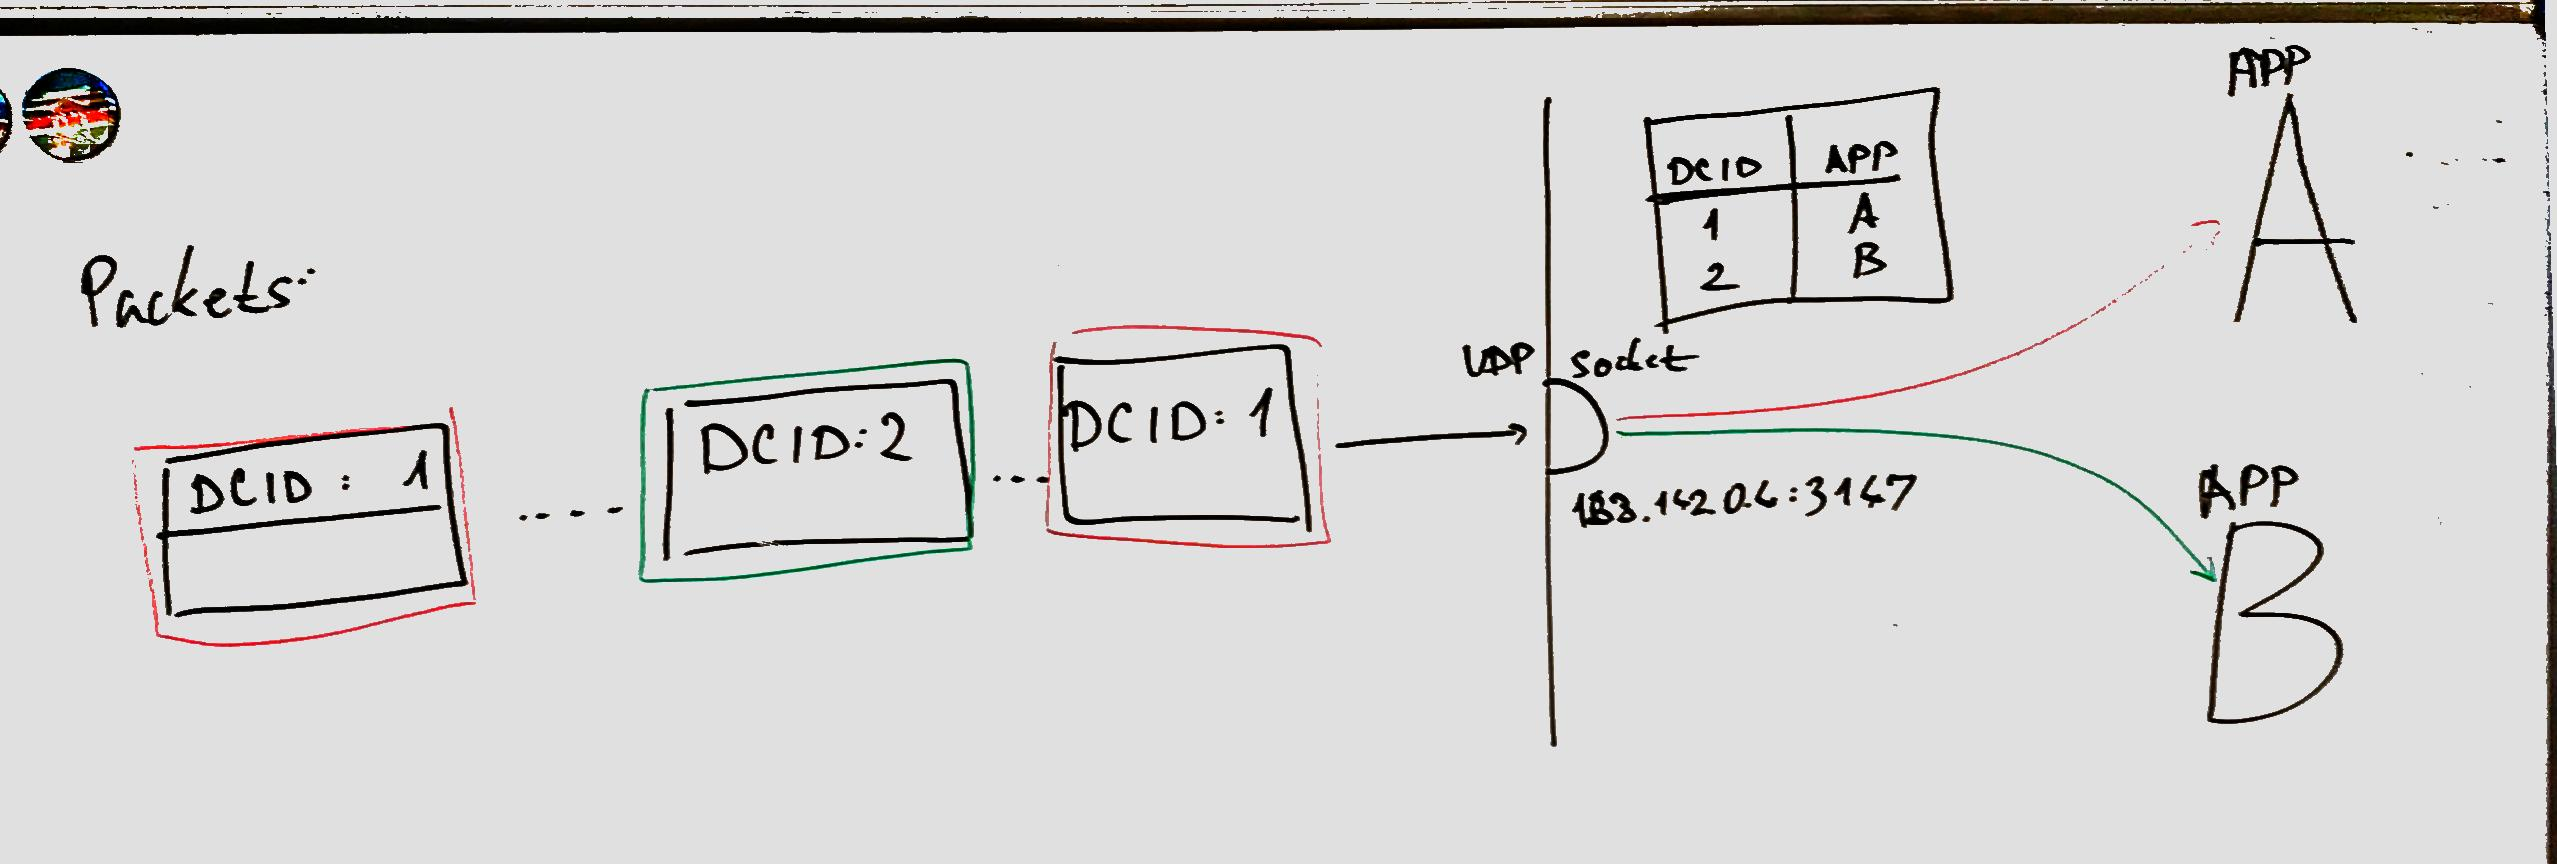
\includegraphics[width=0.9\textwidth]{img/02-socket-multiplexing}
\end{myFigure}

\subsection{QUIC Packets}

QUIC packets sent in the UDP datagram are the smallest processible unit of QUIC\@. The packets are
formed by a header and variable-length payload consisting of one or more QUIC frames. QUIC frames
carry individual pieces of information such as acknowledgements or parts of the streams sent by
the application.

Similarly to TCP, packets in QUIC connections are numbered. However, QUIC uses three separate
\textit{Packet number spaces}:

\begin{enumerate}
  \litem{Initial} Used for exchanging initial information.
  \litem{Handshake} Used during the connection handshake process.
  \litem{1-RTT} Used throughout the lifetime of the connection to transfer application data.
\end{enumerate}

Packets from each packet number space are numbered and processed independently of the other packet
spaces.

\subsection{Packet Encryption}

QUIC packets are encrypted by a symmetric cryptographic cipher. Each packet number space uses
different keys for packet encryption. Initial keys are derived using only the Connection ID chosen
by the client and therefore provide just an obfuscation. Handshake keys are intermediate protection
keys derived during TLS handshake. 1-RTT keys are negotiated by the TLS 1.3 protocol and offer the
same level of security as standard TLS 1.3 connection. The packet encryption is used for protection
both against network traffic observers and against packet payload corruption.

\subsection{Stream Multiplexing}

QUIC can transport multiple streams of data in a single connection. Each stream is identified by its
Stream ID and is processed independently of the other streams. \autoref{fig:02-stream-multiplexing}
illustrates how QUIC may pack two streams into frames such that those streams are transported in
parallel.

\begin{myFigure}{fig:02-stream-multiplexing}{Stream multiplexing in QUIC}
  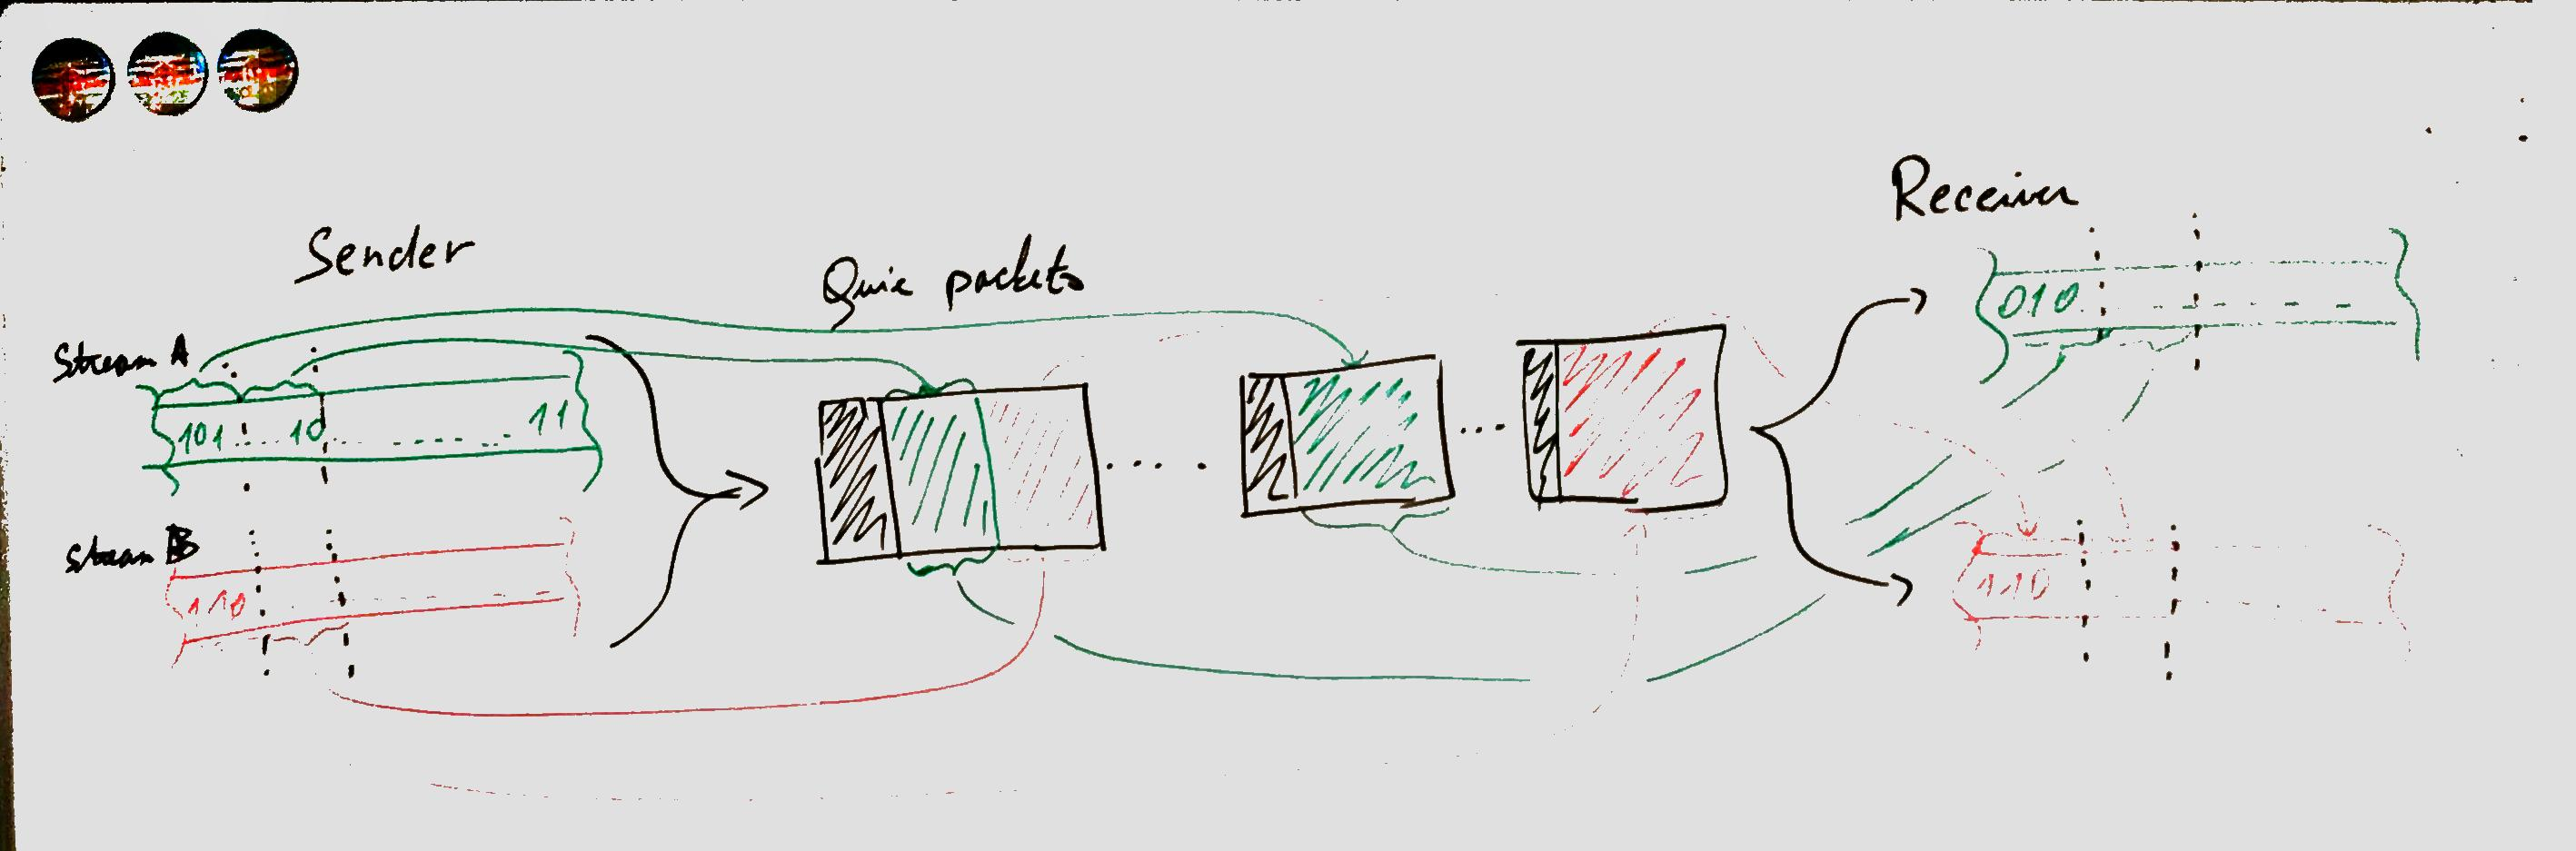
\includegraphics[width=0.9\textwidth]{img/02-stream-multiplexing}
\end{myFigure}

\subsection{Flow Control}

As a prevention against malicious too fast senders, QUIC implements a credit based flow-control
scheme. In this scheme, each peer advertises how much data it is willing to accept and how many
streams of each type can be opened by its peer.

\subsection{Loss Detection and Recovery}

Becuase UDP is an unreliable transport protocol, and QUIC must detect loss of the packets sent. The
loss detection is implemented similarly to TPC via acknowledgements of the received packets.
However, an important difference from TCP is that the lost packet is not retransmitted as-is.
Instead, the data carried by the lost packet are sent in different packets if necessary. This is
illustrated in \autoref{fig:02-packet-loss-example}

\begin{myFigure}{fig:02-packet-loss-example}{Retransmission of lost data in QUIC}
  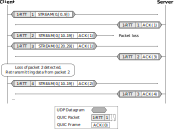
\includegraphics[width=0.6\textwidth]{img/02-retransmission-example}
\end{myFigure}

\subsection{Wire Encoding}

The process of encoding QUIC packets to be sent via the network is optimized for size. All values
sent over the network are encoded in Big-Endian, also known as \textit{network order}. Almost all
numerical values are encoded using a variable-length integer encoding. This encoding uses the two
most significant bits of the first byte to encode whether the value is encoded as 1, 2, 4 or 8 byte
integer. This encoding supports only positive numbers. The ranges available for individual encoding
lengths are listed in \autoref{tab:02-quic-varint-length}.

\begin{myTable}
  {tab:02-quic-varint-length}
  {Variable-length integer encoding lengths}
  {ccr}
  {Most significant bits & Encoding length (B) & Maximum value}
    00                   & 1                   & \num{63}         \\
    01                   & 2                   & \num{16383}      \\
    10                   & 4                   & \num{1073741824} \\
    11                   & 8                   & $2^{62}-1$       \\
\end{myTable}

In order to optimize the size of QUIC packets, the implementations should choose the smallest
possible encoding possible for each encoded number.

\section{QUIC Connection}

In the overview section, we mentioned that QUIC Connections are identified by Connection ID and that
QUIC Packets are exchanged between the endpoints. There are total of five different packet types
that are used in QUIC\@:

\begin{enumerate}
    \litem{Initial \textnormal{and} Handshake} used during connection establishment;

    \litem{1-RTT} main packets used during the lifetime of QUIC connection;

    \litem{Version Negotiation} --- sent by server when client tries to establish connection using
    unsupported version of QUIC\@;

    \litem{0-RTT} carries \textit{early data} when TLS 1.3 0-RTT mode of operation is enabled; and

    \litem{Retry} optionally used by servers for client's address validation when establishing new connections.
\end{enumerate}

Initial, Handshake and 1-RTT packets correspond to the three packet number spaces used throughout
the connection lifetime. For packet processing purposes like acknowledgements and loss detetion, the
1-RTT packet number space also includes 0-RTT packets. Version Negotiation and Retry packets are
used in special cases, are not associated with a packet number space and therefore are neither
encrypted or numbered.

\subsection{QUIC Frames}

Initial, Handshake 0-RTT and 1-RTT frames carry QUIC packets used to transport low-level protocol
messages called QUIC Frames. These frames include e.g.\ ACK frames carrying acknowledgements for
received packets, STREAM frames carrying application data, and CRYPTO frames carrying data for TLS
handshake.

All received QUIC packets have to be acknowledged --- an ACK frame with the packet number must be
sent in an appropriate packet type. However, the frame types carried in the packet determine whether
the acknowledgement has to be sent immediately or if it can be delayed. For example, packets
containing only ACK frames are not acknowledged immediately to avoid unnecessary traffic. Frame
types requiring immediate ack are called \textit{ack-eliciting frames}, and the packets with at
least one such frames are called \textit{ack-eliciting packets}.

There are also restrictions on which frames can be sent in which packets. For example, the STREAM
frames can only be sent in an 1-RTT frames to avoid compromising security.
\autoref{tab:02-frame-types} lists all frame types, whether they are ack-eliciting and in which
packets they can be sent.

\begin{myTable}[\small]
  {tab:02-frame-types}
  {QUIC frame types}
  {l@{\hskip -0.1in}ccccc}
  {Frame type           & Ack-eliciting & Initial      & Handshake    & 0-RTT        & 1-RTT}
PADDING                 &               & \checkmark{} & \checkmark{} & \checkmark{} & \checkmark{} \\
PING                    &               & \checkmark{} & \checkmark{} & \checkmark{} & \checkmark{} \\
ACK                     & \checkmark{}  & \checkmark{} & \checkmark{} &              & \checkmark{} \\
RESET\_STREAM            & \checkmark{}  &              &              & \checkmark{} & \checkmark{} \\
STOP\_SENDING            & \checkmark{}  &              &              & \checkmark{} & \checkmark{} \\
CRYPTO                  & \checkmark{}  & \checkmark{} & \checkmark{} &              & \checkmark{} \\
NEW\_TOKEN               & \checkmark{}  &              &              &              & \checkmark{} \\
STREAM                  & \checkmark{}  &              &              & \checkmark{} & \checkmark{} \\
MAX\_DATA                & \checkmark{}  &              &              & \checkmark{} & \checkmark{} \\
MAX\_STREAM\_DATA         & \checkmark{}  &              &              & \checkmark{} & \checkmark{} \\
MAX\_STREAMS             & \checkmark{}  &              &              & \checkmark{} & \checkmark{} \\
DATA\_BLOCKED            & \checkmark{}  &              &              & \checkmark{} & \checkmark{} \\
STREAM\_DATA\_BLOCKED     & \checkmark{}  &              &              & \checkmark{} & \checkmark{} \\
STREAMS\_BLOCKED         & \checkmark{}  &              &              & \checkmark{} & \checkmark{} \\
NEW\_CONNECTION\_ID       & \checkmark{}  &              &              & \checkmark{} & \checkmark{} \\
RETIRE\_CONNECTION\_ID    & \checkmark{}  &              &              & \checkmark{} & \checkmark{} \\
PATH\_CHALLENGE          & \checkmark{}  &              &              & \checkmark{} & \checkmark{} \\
PATH\_RESPONSE           & \checkmark{}  &              &              & \checkmark{} & \checkmark{} \\
CONNECTION\_CLOSE        &               & \checkmark{} & \checkmark{} & \checkmark{} & \checkmark{} \\
HANDSHAKE\_DONE          & \checkmark{}  &              &              &              & \checkmark{} \\
\end{myTable}

\subsection{Connection Establishment}

QUIC connection is considered establishmed when the TLS handshake is completed. This implies that
both peers have derived the necessary protection keys to be able to receive application data carried
in 1-RTT frames. An example handshake flow is illustrated in
\autoref{fig:02-example-handshake-flow}. The figure lists also the semantics of the content of the
CRYPTO frames sent. However, this is only for illustrative purposes as QUIC does not interpret the
contents of the CRYPTO frames.

\begin{myFigure}
  {fig:02-example-handshake-flow}
  {Example QUIC handshake flow}

  \begin{verbatim}
   Client                                                  Server

   Initial[0]: CRYPTO[CH] ->

                                    Initial[0]: CRYPTO[SH] ACK[0]
                          Handshake[0]: CRYPTO[EE, CERT, CV, FIN]
                                    <- 1-RTT[0]: STREAM[1, "..."]

   Initial[1]: ACK[0]
   Handshake[0]: CRYPTO[FIN], ACK[0]
   1-RTT[0]: STREAM[0, "..."], ACK[0] ->

                               1-RTT[1]: STREAM[3, "..."], ACK[0]
                                          <- Handshake[1]: ACK[0]
  \end{verbatim}
  \todo{Note that this is copied from RFC? Also, this example lacks the HANDSHAKE\_DONE frame}
\end{myFigure}

In it's first datagram, client sends an Initial packet with a single CRYPTO frame contaiting the
\textit{Client Hello} TLS message.

Server replies with a datagram containing three coalesced QUIC packets. The first is an Initial
packet that acknowledgement for the clients Initial packet, and a CRYPTO frame with a \textit{Server
  Hello} message. The contents of the Client Hello are then used to derive Handshake protection keys
and more TLS messages can be sent in the CRYPTO frame in the Handshake packet. The server also has
enough information to derive the 1-RTT keys, so it can also start sending data on Stream 1 using the
STREAM frame in a 1-RTT packet.

Because the servers Initial packet contained an ack-eliciting CRYPTO frame, client needs respond
with another Initial frame with an ACK frame. Contents of the Server Hello message allow client to
derive Handshake protection keys and process the servers Handshake packet. The Handshake packet
needs to be separately acknowledged by an ACK frame and a reply from the TLS layer must be sent in
another CRYPTO frame. By this time, client can also derive 1-RTT protection keys and send or receive
application data in STREAM frames.

\subsection{QUIC packet types}

There are multiple QUIC packet types. These are following:

Payload of Initial, Handshake, and 1-RTT packets contains a sequence of \textit{frames} which are
the low-level messages of the QUIC protocol. Examples of frames include \texttt{STREAM} frames
carrying stream data, \texttt{ACK} frames carrying acknowledgements of received packets and
\texttt{CRYPTO} frames carrying cryptography negotiation messages.
\autoref{fig:streams-frames-and-packets} illustrates how stream data are packaged in frames and
transmitted in packets.

QUIC connections are identified by a connection ID, which is an opaque sequence of 8 to 20 bytes.
Each endpoint sets a value for its peer to include in packets sent towards the endpoint. The
separation of connection identification from endpoint's address eventually allows connection
migration.

\subsection{Handshake and Establishing a Connection}

As mentioned in the introduction, QUIC connection handshake combines TCP's three-way handshake with
TLS protocol handshake. This is achieved by carrying handshake messages of the TLS protocol in
\texttt{CRYPTO} frames. The content of the \texttt{CRYPTO} frames should not be interpreted by QUIC,
only passed to TLS implementation. TLS protocol is also used to negotiate QUIC protocol parameters
via TLS extension parameters and the application-level protocol is negotiated using ALPN
\todo{explain what ALPN is?} protocol.

Similarly to TLS, QUIC packets use increasingly more secure
protection keys for packet encryption.

\begin{itemize}
  \item \textit{Initial keys} are derived from protocol version and Destination Connection ID chosen
    by the client, and are more of an obfuscation rather than protection.
  \item \textit{Handshake keys} are derived during protection secrets exchange by the TLS layer and
    offer intermediate protection.
  \item \textit{1-RTT keys} are derived at the end of TLS handshake and offer strongest
    cryptographic protection.
\end{itemize}

The primary intent of Initial and Handshake packets is transport of \texttt{CRYPTO} frames


Clients initiate new connections by sending an \textit{Initial} QUIC packet. The packet contains a
header with version identifier and random \todo{at least outwardly} source\footnote{Even though
client here chooses both connection IDs, server is allowed choose new destination connection ID to
use and client must accept the change.} and destination connection ID\@. The client inititial packet
carry mainly \texttt{CRYPTO} frames containing TLS \textit{ClientHello} message.

Server replies to the clients initial by sending two packets: Initial packet with an \texttt{ACK}
frame acknowledging the receipt of the clients Initial; and Handshake packet with

\begin{enumerate}
  \item \textit{Version} --- identifier of the version of the protocol used;
  \item \textit{Source Connection ID} and \textit{Destination Connection ID} --- generated randomly
    in a way that can't be predicted by outside observer;
  \item \textit{}
\end{enumerate}

For performance reasons, implementations must the size of UDP datagrams sent in order to avoid
fragmentation at lower network layers. Loss or corruption of a single fragment would lead to entire
UDP datagram being discarded at receivers side. The maximum size, also called maximum transmission
unit (MTU) is dependent on the network and is generally around 1350 bytes.

\subsection{Connection Lifetime}

QUIC packets sent during the connection lifetime are strictly separated into three epochs, called
\textit{packet number spaces} in the specification. QUIC uses slightly different types of packets
for each packet number spaces, and we will refer to packet number spaces using the type of the
packet used in them: \textit{Initial}, \textit{Handshake} and \textit{1-RTT}. The packet number
spaces can be viewed as individual stages of connection establishment.

Packets sent in one packet number space are processed independently of the other packet number
spaces. For example, Acknowledgements for packets sent in \textit{Initial} epoch can only be only
sent in an \textit{Initial} packet. The three packet types also use different protection keys for
packet encryption:

\begin{itemize}

  \item \textit{Initial} --- Keys are derived solely from the protocol version used and the
    Connection ID chosen by the client. This protection is not considered secure, but merely an
    obfuscation.

  \item \textit{Handshake} --- Intermediate protection keys are derived by TLS implementation during
    encryption negotiation and provide partial protection.

  \item \textit{1-RTT} --- Fully secure protection keys are available after finishing connection.
    handshake.

\end{itemize}

Since only 1-RTT packet number space is considered secure, application data can only generally sent
only after connection handshake in 1-RTT packet number space. However, QUIC can optionally allow
sending application data in special \textit{0-RTT} packets. 0-RTT packets belong to 1-RTT packet
number space, but can be sent by client before receiving any packets from server. 0-RTT packet
support requires previous successful connection, and introduces a trade-off between reduced latency
and security.


\section{Streams}

Streams transported by QUIC can be either unidirectional or bidirectional. Unidirectional streams
carry data from initiator to its peer, and bidirectional streams carry data in both directions.
Since both endpoints can open new streams, QUIC recognizes four types of streams. The type of the
stream is encoded in the two least significant bits of the Stream ID, as summarized in
\autoref{tab:02-stream-id-type-map}.

\begin{myTable}
  {tab:02-stream-id-type-map}
  {Mapping of QUIC Stream types to Stream ID bits}
  {cc}
  {Stream type                    & Least significant bits}
  Client-Initiated, Bidirectional  & 00 \\
  Server-Initiated, Bidirectional  & 01 \\
  Client-Initiated, Unidirectional & 10 \\
  Server-Initiated, Unidirectional & 11 \\
\end{myTable}

For example, client initiated unidirectional streams have Stream IDs 2, 6, 10, etc. The Stream ID is
encoded using the variable-length integer encoding and therefore only values 0 to $2^{62}-1$ are
valid.

Bidirectional streams can be viewed as two unidirectional streams combined together. After opening
the stream, each direction of the stream behaves as separate inbound and outbound unidirectional
streams. This means, e.g.\@, that the reading and writing part of the stream can be closed
independently of each other.

Streams are opened simply by starting to sent the stream data. The stream can then be closed by the
writer either by specifying that all data has been written to the stream, or by abruptly terminating
the stream, also called \textit{resetting the stream}. The reader of the stream can request stream
reset in case it no longer wishes to receive data on that stream. Abrupt termination of the stream
requires specifying an application-level error code that will be communicated to the peer.

Implementations should provide a way for application protocols to specify relative priority of
streams.

The implementation should provide following operations on sending part of the stream:

\begin{itemize}

  \item write data;
  \item end the stream by specifying that all data has been written; and
  \item terminate the stream with an application-level error code.

\end{itemize}

On receiving part of the stream, application protocols need to be able to:

\begin{itemize}

  \item read data; and
  \item abort reading with an application-level error code.

\end{itemize}

\todo{do I need schematics of the frames?}

\section{Flow Control}

QUIC aims to be general-purpose transport protocol to be used over potentially untrusted network,
and as such it needs to protect endpoints from malicous peers. One of the mechanisms for achieving
this is limiting the amount of data sender can send and thus preventing overwhelming of slow
receivers by fast senders. Violations of the flow control limits result constitute a protocol
violation and result in an abrupt connection termination.

All QUIC streams are flow controlled individually, and also together as an aggregate. The receiver
controls the maximum amount of data sender can send by specifying

\begin{itemize}
  \item maximum offset of data sent for each individual streams and
  \item maximum sum of all offsets of data sent for individual streams.
\end{itemize}

Additionally, receiver also controls the maximum number of streams the sender can open at any given
moment in order to limit concurrency within a connection.

\begin{itemize}

  \item Streams
  \item Flow control

  \item Connection
    \begin{itemize}
      \item Connection ID,
      \item Packets + Frames intro
      \item Connection establishment
        \begin{itemize}
          \item Encryption + TLS interleaving
          \item  handshake etc.
          \item Other security measures (peer validation)
        \end{itemize}
      \item transport parameters
      \item Connection Termination
    \end{itemize}
  \item Version negotiation
  \item Security
    \begin{itemize}
      \item Other security measures (peer validation)
    \end{itemize}
  \item Packets + Frames
  \item Generating acknowledgements + Recovery

  \item Connection migration?

  \item Detecting maximum packet size
  \item Encoding,
    \begin{itemize}
      \item Variable-length integer
      \item Packet headers, packets, frames, transport parameters
    \end{itemize}

\end{itemize}
